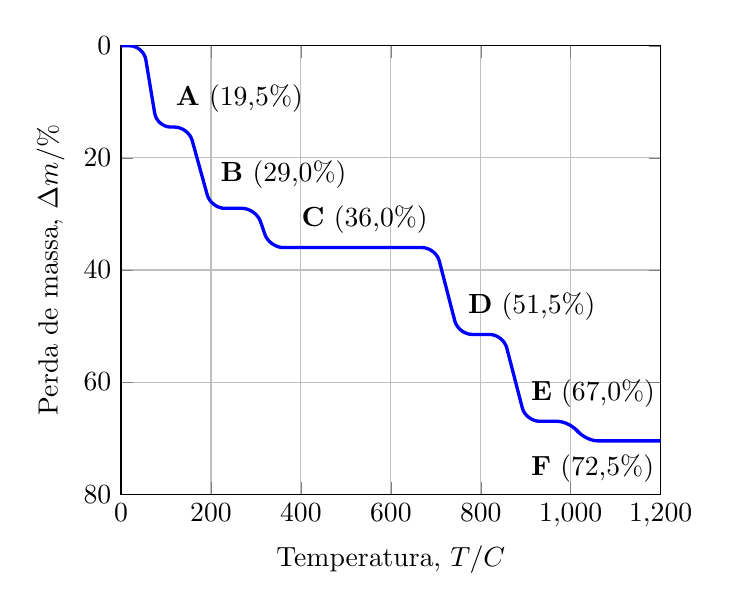
\begin{tikzpicture}
    \begin{axis}
        [
            grid = major,
            ylabel = {Perda de massa, $\Delta m/\%$},
            xlabel = {Temperatura, $T/\unit{\degree C}$},
            xmin = 0, xmax = 1200,
            ymin = 0, ymax = 80,
            y dir=reverse,
        ]
    \draw [draw=blue, very thick, rounded corners=0.5em]
        (axis cs:    0, 00.0) --
        (axis cs:   50, 00.0) --
        (axis cs:   80, 14.5) -- 
        (axis cs:  150, 14.5) -- 
        (axis cs:  200, 29.0) -- 
        (axis cs:  300, 29.0) --
        (axis cs:  330, 36.0) --
        (axis cs:  700, 36.0) --
        (axis cs:  750, 51.5) --
        (axis cs:  850, 51.5) --
        (axis cs:  900, 67.0) --
        (axis cs: 1000, 67.0) --
        (axis cs: 1030, 70.5) --
        (axis cs: 1200, 70.5);
    \node [anchor=west] at (axis cs:  100, 9.5) {\ce{\textbf{A}} (\num{19,5}\%)};
    \node [anchor=west] at (axis cs:  200, 23.0) {\ce{\textbf{B}} (\num{29,0}\%)};
    \node [anchor=west] at (axis cs:  380, 31.0) {\ce{\textbf{C}} (\num{36,0}\%)};
    \node [anchor=west] at (axis cs:  750, 46.5) {\ce{\textbf{D}} (\num{51,5}\%)};
    \node [anchor=west] at (axis cs:  890, 62.0) {\ce{\textbf{E}} (\num{67,0}\%)};
    \node [anchor=west] at (axis cs:  890, 75.5) {\ce{\textbf{F}} (\num{72,5}\%)};
    \end{axis}
 \end{tikzpicture}